\documentclass[a4paper,12pt]{article}

\usepackage[T1]{fontenc}
\usepackage[utf8]{inputenc}
\usepackage[francais]{babel}
\usepackage{multirow,array}
\usepackage{graphicx}
\usepackage{a4wide}
\newcommand{\HRule}{\rule{\linewidth}{1mm}}

\begin{document}


%
%  TITRE
%

\begin{titlepage}

\begin{center}
\huge Localisation géométrique rapide \\ par arbre octal
\HRule \\
\medskip
{\Huge \bfseries La librairie libOL} \\
\HRule
\end{center}

\vspace*{\stretch{3}}

\begin{figure}[htbp]
\begin{center}
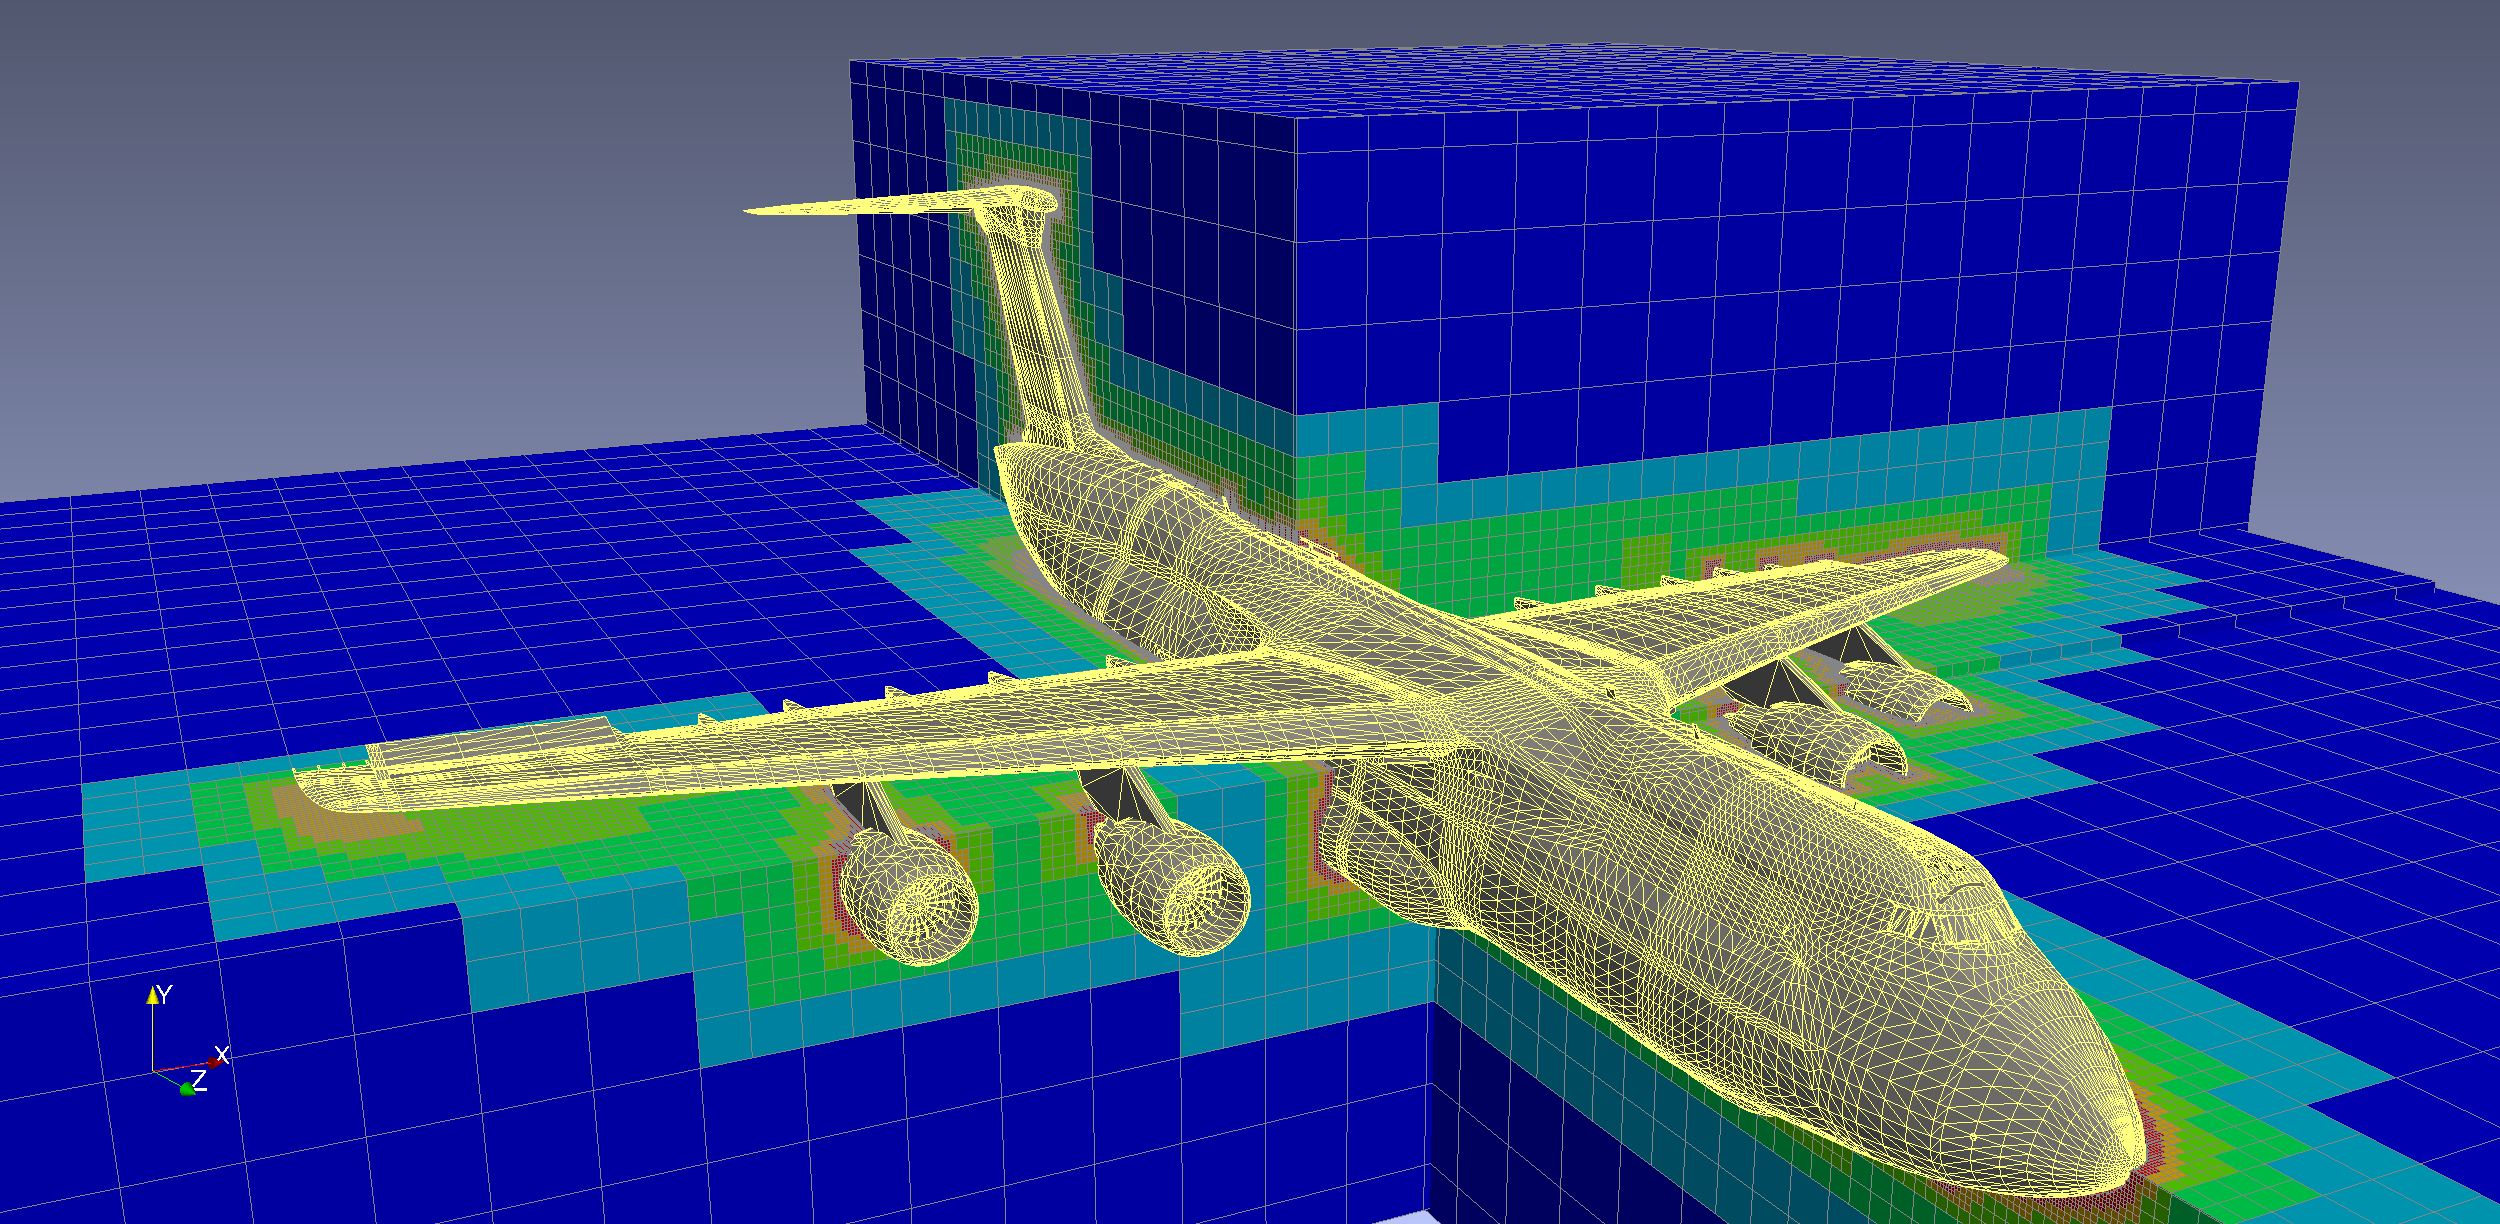
\includegraphics[height=7.8cm]{octree_mesh.png}
\end{center}
\end{figure}

\vspace*{\stretch{1}}

\begin{flushright}
\Large Lo\"ic MAR\'ECHAL / INRIA, Projet Gamma\\
\Large Février 2024 \\
\normalsize Document v1.52, librairie v1.82
\end{flushright}

\end{titlepage}

\clearpage

\setcounter{tocdepth}{2}
\tableofcontents
\vfill

\footnotesize{Couverture : Maillage octree d'un Boeing 747 réalisé par Thomas Døhlen.}
\normalsize

\clearpage


%
%  1 / INTRODUCTION
%

\section{Introduction}
Le but de cette librairie est de facilement et rapidement retrouver certains éléments d'un maillage en effectuant des requêtes géométriques, telles que trouver le triangle le plus proche d'un point donné, ou bien de fournir la liste des triangles ou sommets inclus dans une zone rectangulaire donnée.

D'autres entités que les triangles ou sommets sont gérés tels que les arêtes, les quadrilatères et tétraèdres.

L'utilisateur a le moyen de définir des fonctions filtres afin de contraindre les critères de recherches à son propre contexte.

Une des principales forces de cette librairie est sa très grande efficacité tant en termes de mémoire, les données utilisateur ne sont pas dupliquées et l'arbre est encodé sous forme binaire, que de temps de calcul, l'appel des requêtes étant \emph{thread-safe} et peut donc être appelé en parallèle.

%
%  2 / UTILISATION
%

\section{Utilisation}
La donnée d'entrée à fournir à la librairie est un maillage de surface ou de volume sous sa forme la plus simple : une liste des coordonnées de chaque sommet et une table des numéros des sommets pour chaque élément. À partir de ce maillage, la librairie génère un octree automatiquement raffiné de telle sorte que chaque octant ne contienne au plus que 20 entités de chaque type afin d'accélérer les opérations de recherche. Le temps de construction et la mémoire requis sont donc dépendants du nombre d'entités du maillage et de la forme de la géométrie. Un octree étant fondamentalement isotrope, il aura tendance à être fortement raffiné, et donc à occuper beaucoup de mémoire, dans le cas de géométries très minces (anisotropes).

Bien qu'une structure octree ne contienne qu'un seul maillage, il est possible d'en créer plusieurs, ceux-ci étant différenciés par une étiquette unique retournée à la création.

Supposons que nous aillons un maillage de \emph{NmbVer} sommets, stockés dans la table \emph{VerCrd} et \emph{NmbTri} triangles dans la table \emph{TriTab} et que l'on souhaite trouver le triangle le plus proche du point de coordonnées $\{0.5, 2.3, -6.0\}$ ainsi que la liste des triangles contenus partiellement ou totalement dans la région cubique centrée en $\{2,2,10\}$ et de taille $2$. Le déroulement est le suivant :

\begin{tt}
\begin{verbatim}
int64_t OctIdx;
int IntersectedTriangles[10];
int NmbVer, NmbTri, (*TriTab)[3];
double (*CrdTab)[3], VerCrd[3]={0.5, 2.3, -6.0};
double BoxMin[3]={1,1,9}, BoxMax[3]={3,3,11}, MinDis;
...
(allocation et lecture du maillage)
...
OctIdx = LolNewOctree(
         NmbVer, VerTab[1], VerTab[2],
              0,      NULL,      NULL,
         NmbTri, TriTab[1], TriTab[1],
              0,      NULL,      NULL,
              0,      NULL,      NULL,
              0,      NULL,      NULL,
              0,      NULL,      NULL,
              0,      NULL,      NULL,
              1, 1);

printf("l'Octree numéro %d a été construit\n", OctIdx);

TriIdx = LolGetNearest(OctIdx, TypTri, VerCrd, &MinDis, 0, NULL, NULL, 0);
printf("le triangle le plus proche de 0.5, 2.3, -6.0 est : %d\n", TriIdx);

NmbBoxTri = LolGetBoundingBox(OctIdx, TypTri, 10, TriTab, BoxMin, BoxMax, 0);
for(i=0;i<NmbTri;i++)
    printf("triangle numéro : %d\n", TriTab[i]);

LolFreeOctree(OctIdx);
\end{verbatim}
\end{tt}
\normalfont

Il est à noter que l'intersection d'un triangle avec une boîte est calculée de manière complète, c'est-à-dire qu'il y a intersection si l'un des sommets du triangle tombe dans la boîte, ou qu’une de ses arêtes intersecte une face de la boîte ou encore que le plan du triangle intersecte une arête de la boîte. Certains octrees simplifiés se contentent de tester si un sommet de triangle est contenu dans la boîte, l'approche de la libOL est plus consommatrice de ressource, mais est géométriquement exact.

La vitesse de création est d'environ 2.000.000 de sommets ou 200.000 triangles par seconde et la consommation mémoire de 30 octets par sommet ou 240 octets par triangle.

La librairie étant constituée d'un seul fichier {\tt liboctree.c} et d'un fichier de définitions {\tt liboctree.h} pour le C et {\tt liboctree.ins}.

Note : par défaut la librairie utilise des entiers codés sur 32 bits, mais il est possible de les étendre à 64 bits en passant le paramètre {\tt -Di8} au compilateur.


%
%  3 / COMMANDES
%

\clearpage
\section{Liste des commandes}


\subsection{LolFreeOctree}
Libère un octree et toute la mémoire associée à cette instance. Cela ne clôture pas la librairie qui peut continuer à allouer d'autres instances.

\subsubsection*{Syntaxe}
{\tt mem = LolFreeOctree(OctIdx);}

\subsubsection*{Commentaires}
Retourne la mémoire totale utilisée en octets.


\subsection{LolGetBoundingBox}
Retourne une liste d'entités de maillage d'un type donné et inclus dans une boîte englobante.

\subsubsection*{Syntaxe}
\begin{tt}
\begin{verbatim}
NmbTri = LolGetBoundingBox(
         OctIdx, typ, MaxTri, TriTab,
         BoxMin[3], BoxMax[3], ThrIdx);}
\end{verbatim}
\end{tt}
\normalfont

\subsubsection*{Paramètres}
\begin{tabular}{|m{3cm}|m{2cm}|m{8.5cm}|}
\hline
Paramètre  & type      & description \\
\hline
OctIdx     & int64\_t  & index de l'octree retourné par LolNewOctree \\
\hline
typ        & int       & type d'entité à rechercher: LolTypVer, LolTypEdg, LolTypTri, LolTypQad ou LolTypTet \\
\hline
MaxTri     & int       & nombre maximum d'éléments que la table suivante peut contenir \\
\hline
TriTab     & int *     & pointeur sur une table qui contiendra la liste des éléments contenus dans cette boîte englobante \\
\hline
BoxMin     & double [3] & coordonnées du coin inférieur de la boîte englobante \\
\hline
BoxMin     & double [3] & coordonnées du coin supérieur de la boîte englobante \\
\hline
ThrIdx     & int        & numéro du thread ou process appelant ou 0 dans le cas séquentiel \\
\hline
\end{tabular}

\medskip

\begin{tabular}{|m{3cm}|m{2cm}|m{8.5cm}|}
\hline
Retour     & type   & description \\
\hline
index      & int    & retourne le nombre d'entités contenues dans la boîte \\
\hline
\end{tabular}

\subsubsection*{Exemple}
Alloue une table de 10 triangles et demande à la librairie de retourner les 10 premiers triangles intersectant le cube de coordonnés $\{0,0,0\} - \{1,1,1\}$ et affiche leur numéro.

\begin{tt}
\begin{verbatim}
int TriTab[10];
double box[2][3]={{0,0,0}, {1,1,1}};
NmbTri = LolGetBoundingBox(OctIdx, TypTri, 10, TriTab, box[0], box[1], 0);
for(i=0;i<NmbTri;i++)
    printf("triangle numéro : %d\n", TriTab[i]);
\end{verbatim}
\end{tt}
\normalfont


\subsection{LolGetNearest}
Recherche l'entité de type spécifiée la plus proche d'une coordonnée géométrique.

\subsubsection*{Syntaxe}
\begin{tt}
\begin{verbatim}
index = LolGetNearest(
        OctIdx, typ, crd, PtrMinDis, MaxDis,
        UsrPrc, UsrDat, ThrIdx);}
\end{verbatim}
\end{tt}
\normalfont

\subsubsection*{Paramètres}
\begin{tabular}{|m{3cm}|m{2cm}|m{8.5cm}|}
\hline
Paramètre  & type       & description \\
\hline
OctIdx     & int64\_t   & index de l'octree retourné par LolNewOctree \\
\hline
typ        & int        & type d'entité à rechercher: LolTypVer, LolTypEdg, LolTypTri, LolTypQad ou LolTypTet \\
\hline
crd        & double [3] & coordonnées du vertex de référence \\
\hline
PtrMinDis  & double *   & pointeur sur une valeur dans laquelle la distance à l'entité la plus proche sera retournée \\
\hline
MaxDis     & double     & limiter la recherche à des entités distance au maximum de MaxDis du point de référence (0 si aucune limite n'est souhaitée) \\
\hline
UsrPrc     & int ()(void *, int) & pointeur sur une routine de filtrage prenant en entré un pointeur sur les données utilisateur et un entier contenant l'entité en cours de test et qui retourne un entier booléen : 0 pour exclure du test et 1 pour effectuer le test \\
\hline
UsrDat     & void *    & pointeur sur les données de l'utilisateur qui sera transmis à la routine de test \\
\hline
ThrIdx     & int        & numéro du thread ou process appelant ou 0 dans le cas séquentiel \\
\hline
\end{tabular}

\medskip

\begin{tabular}{|m{3cm}|m{2cm}|m{8.5cm}|}
\hline
Retour     & type   & description \\
\hline
index      & int    & retourne l'index de l'entité la plus proche du sommet de référence fourni ou 0 en cas d'erreur \\
\hline
\end{tabular}
\subsubsection*{Commentaires}
Il est tout à fait possible de donner un point de référence en dehors de la boîte englobante de l'octree qui est taillé au plus juste autour de l'objet fourni en entrée. Plus le point est éloigné du triangle le plus proche, plus le temps de recherche sera long.

La routine de filtrage optionnelle est appelée en aveugle avec comme premier paramètre le pointeur {\tt UsrDat} fourni par l'utilisateur en tant que {\tt void *}, et le numéro de l'entité de maillage que la librairie souhaite évaluer au cours d'une requête. Le rôle de cette routine est de retourner un résultat booléen, 0 pour refuser de considérer cette entité dans la liste à tester et 1 pour l'envoyer au test.

L'index {\tt ThrIdx} est un identifiant unique du process ou thread de l'utilisateur qui appellent la procédure de recherche et dont le numéro doit être compris entre $0$ et $MaxThr-1$ où $MaxThr$ est le nombre maximum de processus pouvant appeler les fonctions de la librairie de manière concurrente.

L'exemple suivant génère un octree autour d'un maillage de quatre sommets et deux triangles et cherche lequel des deux est le plus proche du point d'origine $\{0,0,0\}$.

\subsubsection*{Exemple}

\begin{tt}
\begin{verbatim}
double crd[5][3] = { {2,-3,5.2}, {3.4,6,8.2}, {5,1,3}, {3,4,1}, {0,0,0} };
double MinDis;
int tri[2][3] = { {1,2,3}, {2,3,4} };
OctIdx = LolNewOctree(4, crd[0], crd[1], 2, tri[0], tri[1], 0);
TriIdx = LolGetNearest(OctIdx, TypTri, crd[4], &MinDis, 0, NULL, NULL, 0);
printf("le triangle le plus proche de l'origine est %d\n", TriIdx);
\end{verbatim}
\end{tt}
\normalfont


\subsection{LolIntersectSurface}
Recherche le premier triangle intersecté par le vecteur donné. Cette routine, qui ne fonctionne pour l'instant qu'avec les triangles, permet de rechercher une entité proche, mais par lancer de rayon plutôt que par distance comme LolGetNearest().

\subsubsection*{Syntaxe}
\begin{tt}
\begin{verbatim}
index = LolIntersectSurface(
        OctIdx, crd, tng, PtrMinDis, MaxDis,
        UsrPrc, UsrDat, ThrIdx);}
\end{verbatim}
\end{tt}
\normalfont

\subsubsection*{Paramètres}
\begin{tabular}{|m{3cm}|m{2cm}|m{8.5cm}|}
\hline
Paramètre  & type       & description \\
\hline
OctIdx     & int64\_t   & index de l'octree retourné par LolNewOctree \\
\hline
crd        & double [3] & coordonnées du point d'origine du vecteur \\
\hline
tng        & double [3] & tangente du vecteur \\
\hline
PtrMinDis  & double *   & pointeur sur une valeur dans laquelle la distance à l'entité la plus proche sera retournée \\
\hline
MaxDis     & double     & limiter la recherche à des entités distance au maximum de MaxDis du point de référence (0 si aucune limite n'est souhaitée) \\
\hline
UsrPrc     & int ()(void *, int) & pointeur sur une routine de filtrage prenant en entré un pointeur sur les données utilisateur et un entier contenant l'entité en cours de test et qui retourne un entier booléen : 0 pour exclure du test et 1 pour effectuer le test \\
\hline
UsrDat     & void *    & pointeur sur les données de l'utilisateur qui sera transmis à la routine de test \\
\hline
ThrIdx     & int       & numéro du thread ou process appelant ou 0 dans le cas séquentiel \\
\hline
\end{tabular}

\medskip

\begin{tabular}{|m{3cm}|m{2cm}|m{8.5cm}|}
\hline
Retour     & type   & description \\
\hline
index      & int    & retourne l'index de l'entité la plus proche intersecté par le vecteur fourni ou 0 en cas d'erreur \\
\hline
\end{tabular}
\subsubsection*{Commentaires}
Il est tout à fait possible de donner un point de référence en dehors de la boîte englobante de l'octree qui est taillé au plus juste autour de l'objet fourni en entrée. Plus le point est éloigné du triangle le plus proche, plus le temps de recherche sera long.

La routine de filtrage optionnelle est appelée en aveugle avec comme premier paramètre le pointeur {\tt UsrDat} fourni par l'utilisateur en tant que {\tt void *}, et le numéro de l'entité de maillage que la librairie souhaite évaluer au cours d'une requête. Le rôle de cette routine est de retourner un résultat booléen, 0 pour refuser de considérer cette entité dans la liste à tester et 1 pour l'envoyer au test.

L'index {\tt ThrIdx} est un identifiant unique du process ou thread de l'utilisateur qui appellent la procédure de recherche et dont le numéro doit être compris entre $0$ et $MaxThr-1$ où $MaxThr$ est le nombre maximum de processus pouvant appeler les fonctions de la librairie de manière concurrente.


\clearpage
\subsection{LolNewOctree}

\subsubsection*{Syntaxe}
\begin{tt}
\begin{verbatim}
retour = LolNewOctree(
         NmbVer, pVer1, pVer2,
         NmbEdg, pEdg1, pEdg2,
         NmbTri, pTri1, pTri2,
         NmbQad, pQad1, pQad2),
         NmbTet, pTet1, pTet2,
         NmbPyr, pPyr1, pPyr2,
         NmbPri, pPri1, pPri2,
         NmbHex, pHex1, pHex2,
         BasIdx, MaxThr);}
\end{verbatim}
\end{tt}
\normalfont

\subsubsection*{Paramètres}

\begin{tabular}{|m{2cm}|m{2cm}|m{10cm}|}
\hline
Paramètre  & type     & description \\
\hline
NmbVer     & int      & nombre de sommets à insérer dans l'octree \\
\hline
pVer1      & double * & pointeur sur la table des coordonnées du premier sommet du maillage \\
\hline
pVer1      & double * & pointeur sur la table des coordonnées du second sommet du maillage \\
\hline
\end{tabular}

\begin{tabular}{|m{2cm}|m{2cm}|m{10cm}|}
\hline
NmbEdg     & int      & nombre d'arêtes à insérer dans l'octree  \\
\hline
pEdg1      & int *    & pointeur sur la table des indices de sommets de la première arête du maillage \\
\hline
pEdg2      & int *    & pointeur sur la table des indices de sommets de la seconde arête du maillage \\
\hline
NmbTri     & int      & nombre de triangles à insérer dans l'octree  \\
\hline
pTri1      & int *    & pointeur sur la table des indices de sommets du premier triangle du maillage \\
\hline
pTri2      & int *    & pointeur sur la table des indices de sommets du second triangle du maillage \\
\hline
NmbQad     & int      & nombre de quads à insérer dans l'octree  \\
\hline
pQad1      & int *    & pointeur sur la table des indices de sommets du premier quad du maillage \\
\hline
pQad2      & int *    & pointeur sur la table des indices de sommets du second quad du maillage \\
\hline
\end{tabular}

\begin{tabular}{|m{2cm}|m{2cm}|m{10cm}|}
\hline
NmbTet     & int      & nombre de tétraèdres à insérer dans l'octree  \\
\hline
pTet1      & int *    & pointeur sur la table des indices de sommets du premier tétraèdre du maillage \\
\hline
pTet2      & int *    & pointeur sur la table des indices de sommets du second tétraèdre du maillage \\
\hline
NmbPyr     & int      & nombre de pyramides à insérer dans l'octree  \\
\hline
pPyr1      & int *    & pointeur sur la table des indices de sommets de la première pyramide du maillage \\
\hline
pPyr2      & int *    & pointeur sur la table des indices de sommets de la seconde pyramide du maillage \\
\hline
NmbPri     & int      & nombre de prismes à insérer dans l'octree  \\
\hline
pPri1      & int *    & pointeur sur la table des indices de sommets du premier prisme du maillage \\
\hline
pPri2      & int *    & pointeur sur la table des indices de sommets du second prisme du maillage \\
\hline
NmbHex     & int      & nombre d'hexaèdres à insérer dans l'octree  \\
\hline
pHex1      & int *    & pointeur sur la table des indices de sommets du premier hexaèdre du maillage \\
\hline
pHex2      & int *    & pointeur sur la table des indices de sommets du second hexaèdre du maillage \\
\hline
BasIdx     & int      & index de l'indice de début de chaque table : 0 ou 1 \\
\hline
MaxThr     & int      & nombre maximum de processus ou thread pouvant effectuer des requêtes de manière concurrente sur cet octree : vaut 1 ou plus \\
\hline
\end{tabular}

\medskip

\begin{tabular}{|m{2cm}|m{2cm}|m{10cm}|}
\hline
Retour     & type   & description \\
\hline
index      & int    & retourne l'index d'un octree à fournir aux commandes de la librairie ou 0 en cas d'erreur \\
\hline
\end{tabular}
\subsubsection*{Commentaires}
Si vous avez du mal à jongler avec les déclarations de tableaux multidimensionnels, plutôt cryptiques, du C, vous pouvez passer un simple tableau unidimensionnel de double (double *), où VerTab[0] est la coordonnée $x_1$ du premier vertex, VerTab[1] est $y_1$, VerTab[2] est $z_1$, VerTab[3] est $x_2$ et ainsi de suite.
Notez que la mémoire prise par l'octree dépend aussi du paramètre MaxThr, car une petite quantité de mémoire de travail est allouée pour chaque thread (plus 10\%).
De plus, si vous compilez la librairie en passant l'option {\tt -DWITH\_FAST\_MODE} au compilateur, la structure octree occupera 2,5 fois plus de mémoire, mais toutes les requêtes seront 35\% plus rapides.

L'exemple suivant génère un octree autour d'un maillage de quatre sommets et deux triangles.

\subsubsection*{Exemple}

\begin{tt}
\begin{verbatim}
double crd[4][3] = { {2,-3,5.2}, {3.4,6,8.2}, {5,1,3}, {3,4,1} };
int tri[2][3] = { {1,2,3}, {2,3,4} };
OctIdx = LolNewOctree(
         4, crd[0], crd[1],
         0, NULL, NULL,
         2, tri[0], tri[1]);
         0, NULL, NULL,
         0, NULL, NULL,
         0, NULL, NULL,
         0, NULL, NULL,
         0, NULL, NULL,
         0, 1);
\end{verbatim}
\end{tt}
\normalfont


\subsection{LolProjectVertex}
Projection géométrique et topologique d'un point sur une entité de maillage. La distance et le projeté sur une arrête, un triangle, un quadrilatère ou un tétraèdre est calculé, ainsi que la nature de ce projeté, si le projeté se confond exactement avec le sommet ou l'arrête d'un triangle par exemple.

\subsubsection*{Syntaxe}
{\tt statut = LolProjectVertex(OctIdx, VerCrd, SrfTyp, SrfIdx, PrjCrd, ThrIdx);}

\subsubsection*{Paramètres}
\begin{tabular}{|m{3cm}|m{2cm}|m{8.5cm}|}
\hline
Paramètre  & type       & description \\
\hline
OctIdx     & int64\_t   & index de l'octree retourné par LolNewOctree \\
\hline
VerCrd     & double [3] & coordonnées du vertex à projeter \\
\hline
SrfTyp     & int        & type d'entité sur laquelle projeter le vertex : LolTypVer, LolTypEdg, LolTypTri, LolTypQad ou LolTypTet \\
\hline
SrfIdx     & int        & index de l'entité de surface \\
\hline
PrjCrd     & double [3] & pointeur sur les coordonnées qui recevront la projection \\
\hline
ThrIdx     & int        & numéro du thread ou process appelant ou 0 dans le cas séquentiel \\
\hline
\end{tabular}

\medskip

\begin{tabular}{|m{3cm}|m{2cm}|m{8.5cm}|}
\hline
Retour     & type   & description \\
\hline
statut     & int    & 0 : erreur, 1 : projection confondue avec un vertex, 2 : idem avec une edge, 3 : projection à l'intérieur du triangle ou quadrilatère \\
\hline
\end{tabular}

\end{document}
